\cleardoublepage
\chapter{Neurophysiological and behavioral factors associated with a high DRF}
\label{disc:drf}

\section{Summary of the results}
\label{disc:drf:summary}

\begin{figure}[htb]
	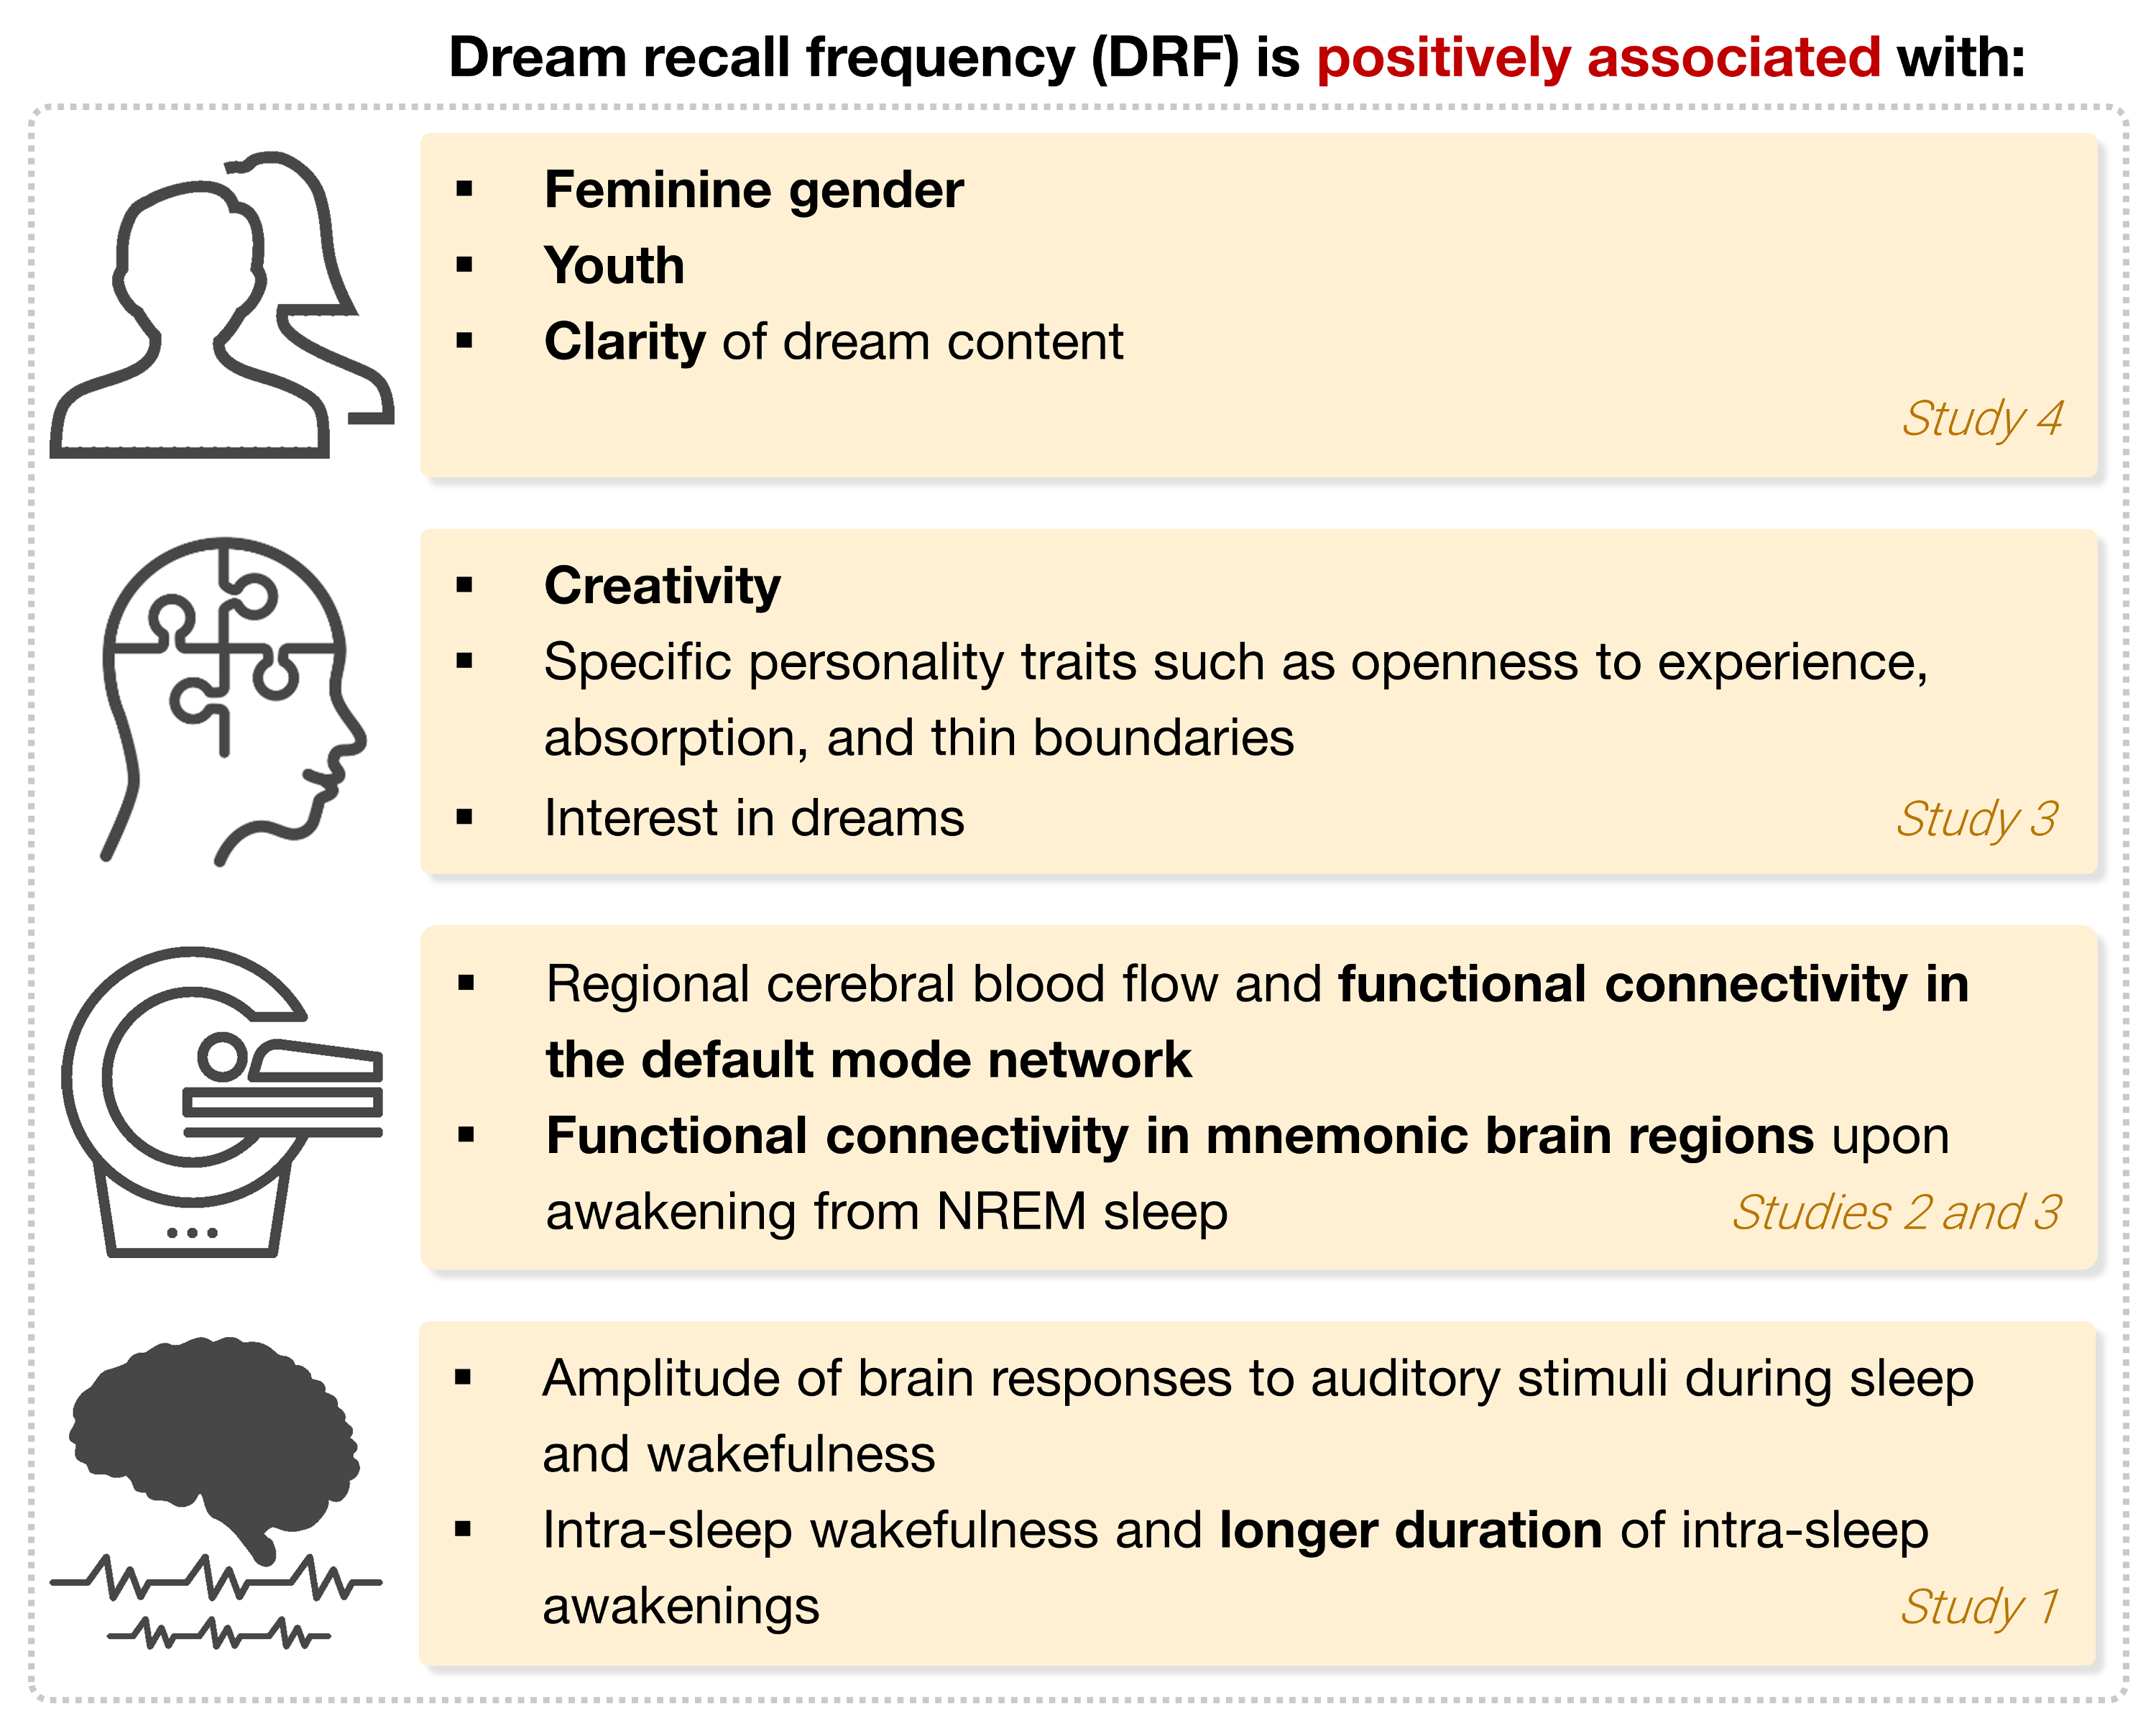
\includegraphics[width=\textwidth]{Fig/Discussion/HR_recap.png}
	\caption[Summary of the results on DRF]{Summary of the behavioral and neurophysiological differences observed between high and low dream recallers}
	\label{fig:disc:drf:summary}
\end{figure}


%%%%%%%%%%%%%%%%%%%%%%%%%%%%%%%%%%%%%%%%%%%%%%%%%%%%%%%%%%%%%%%%%%%%%%%%%%%%%%%
\cleardoublepage
\chapter{The relationship between waking life and dream content}
\label{disc:wle}

%%%%%%%%%%%%%%%%%%%%%%%%%%%%%%%%%%%%%%%%%%%%%%%%%%%%%%%%%%%%%%%%%%%%%%%%%%%%%%%
\cleardoublepage
\chapter{Methodological development}
\label{disc:methods}

\section{A state-of-the-art open-source software}
\label{disc:methods:software}

SLEEP is a free, cross-platform and open-source graphical user interface dedicated to sleep reading, scoring and analysis. Initially designed for a personal use, it soon extended into a fully developed module with a comprehensive and intuitive interface. SLEEP has many advantages over other existing solutions. First, and perhaps most importantly, it is free and open-source. Second, it leverages the graphics processing unit to deliver cutting edge graphical performances. Third, it natively supports several commercial and public data file formats, thus making it accessible to the greatest possible number of people. Fourth, it implements several signal processing tools, as well as several automatic detections of sleep microstructural features. Fifth, it comes with an extensive documentation, a chat room and a peer-reviewed publication. In view of all these functionalities, one can reasonably conclude that SLEEP represents a state-of-the-art software in sleep research which should consequently benefit many. Furthermore, as the development of the software is still ongoing, novel functionalities will continue to be added. Some of these future perspectives are detailed in the section below.

\section{Future directions}
\label{disc:methods:future}

SLEEP includes so far 6 algorithms for detecting some of the most prominent features of each sleep stage, namely spindles, K-complexes, slow waves, rapid eye movements and muscle twitches. Two of these detections (i.e. spindles and K-complexes) were compared against a visual scoring reference and showed overall good performances. Yet, there are still opportunities for further enhancements and the detection algorithms were improved since the initial, published, version. An example of the updated spindles detection can be found in Figure \ref{fig:disc:methods:future:spindles}.

\begin{figure}[htb]
	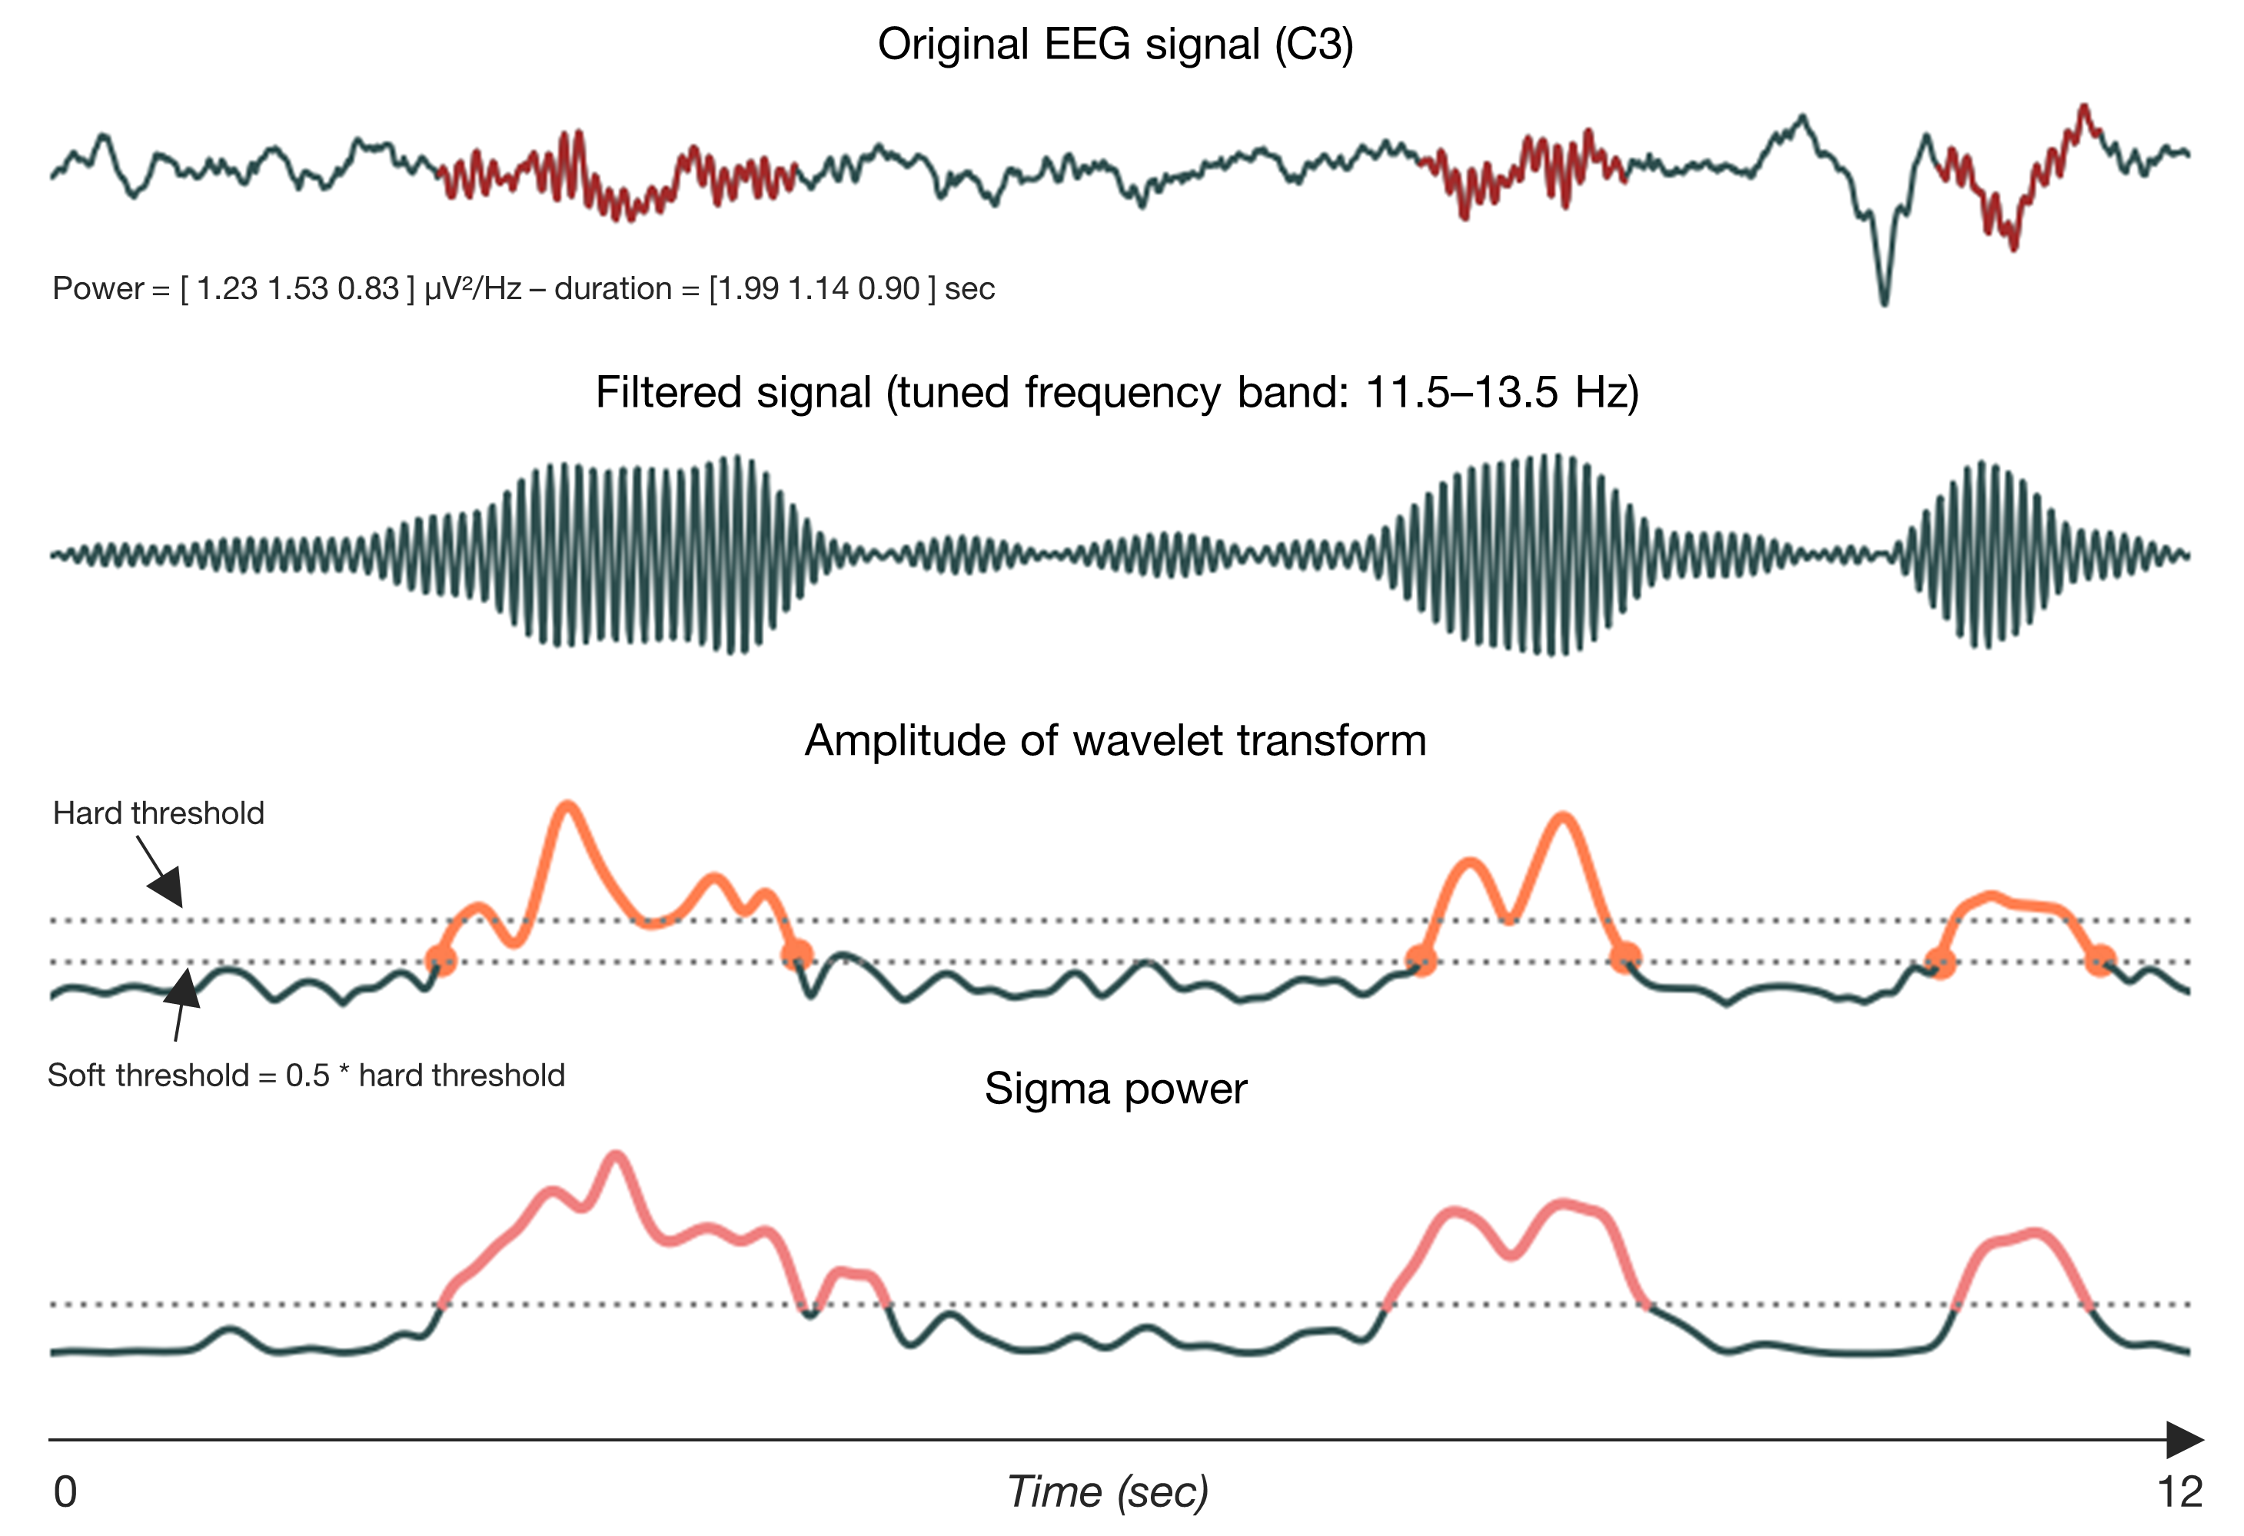
\includegraphics[width=\textwidth]{Fig/Discussion/spindles.png}
	\caption[Improved spindles detection algorithm]{Improved spindles detection algorithm. Compared to the initial algorithm (presented in chapter \ref{res:software}), the new spindles detection has several improvements. First, we implemented a data-driven tuning of the spindle frequency band by finding the peak spectral power within the sigma range. This step, described by \citet{berthomier_automatic_2007}, allows to accommodate for inter-individual variability of EEG signals, and is particularly useful when analyzing patients who tend to exhibit higher variability. Second, we now use both a hard and a soft threshold on the amplitude of the wavelet transform to determine more precisely the beginning and the end of each spindle. Finally, to allow users to better understand how the detection algorithm works, we implemented a function to plot the current figure for each desired time window.}
	\label{fig:disc:methods:future:spindles}
\end{figure}

Perhaps one of the most challenging issue in sleep research is the scoring of sleep stages. Currently, the gold standard remains visual scoring by an expert, which is time-consuming and subject to high inter-rater variability. There is therefore a crucial need for reliable and time-efficient algorithms capable of detecting sleep stages in healthy and patients alike. While recent years have witnessed a surge in automatic sleep scoring methods (e.g. \citealp{berthomier_automatic_2007, lajnef_learning_2015}), there is always a room for improvement and one of the ultimate goal of SLEEP software would therefore be to embed within the graphical user interface a function to perform automatic sleep scoring.

With this in mind, we are currently working on two distinct automatic sleep scoring methods, based on spectral feature extraction / microstructural detection (Fig \ref{fig:disc:methods:future:auto:autoscore}), and on machine-learning algorithms, respectively. Preliminary results based on the former method show a 81\% agreement with a manually scored standard reference, a figure comprised within the range of human inter-scorer agreements (generally between 80 and 90\%, see \citealp{silber_visual_2007}). A similar agreement was obtained using the second, machine-learning based automatic sleep scoring method. Future developments will be needed to get the most out of these two methods to provide a state-of-the-art algorithm.

\begin{figure}[htb]
	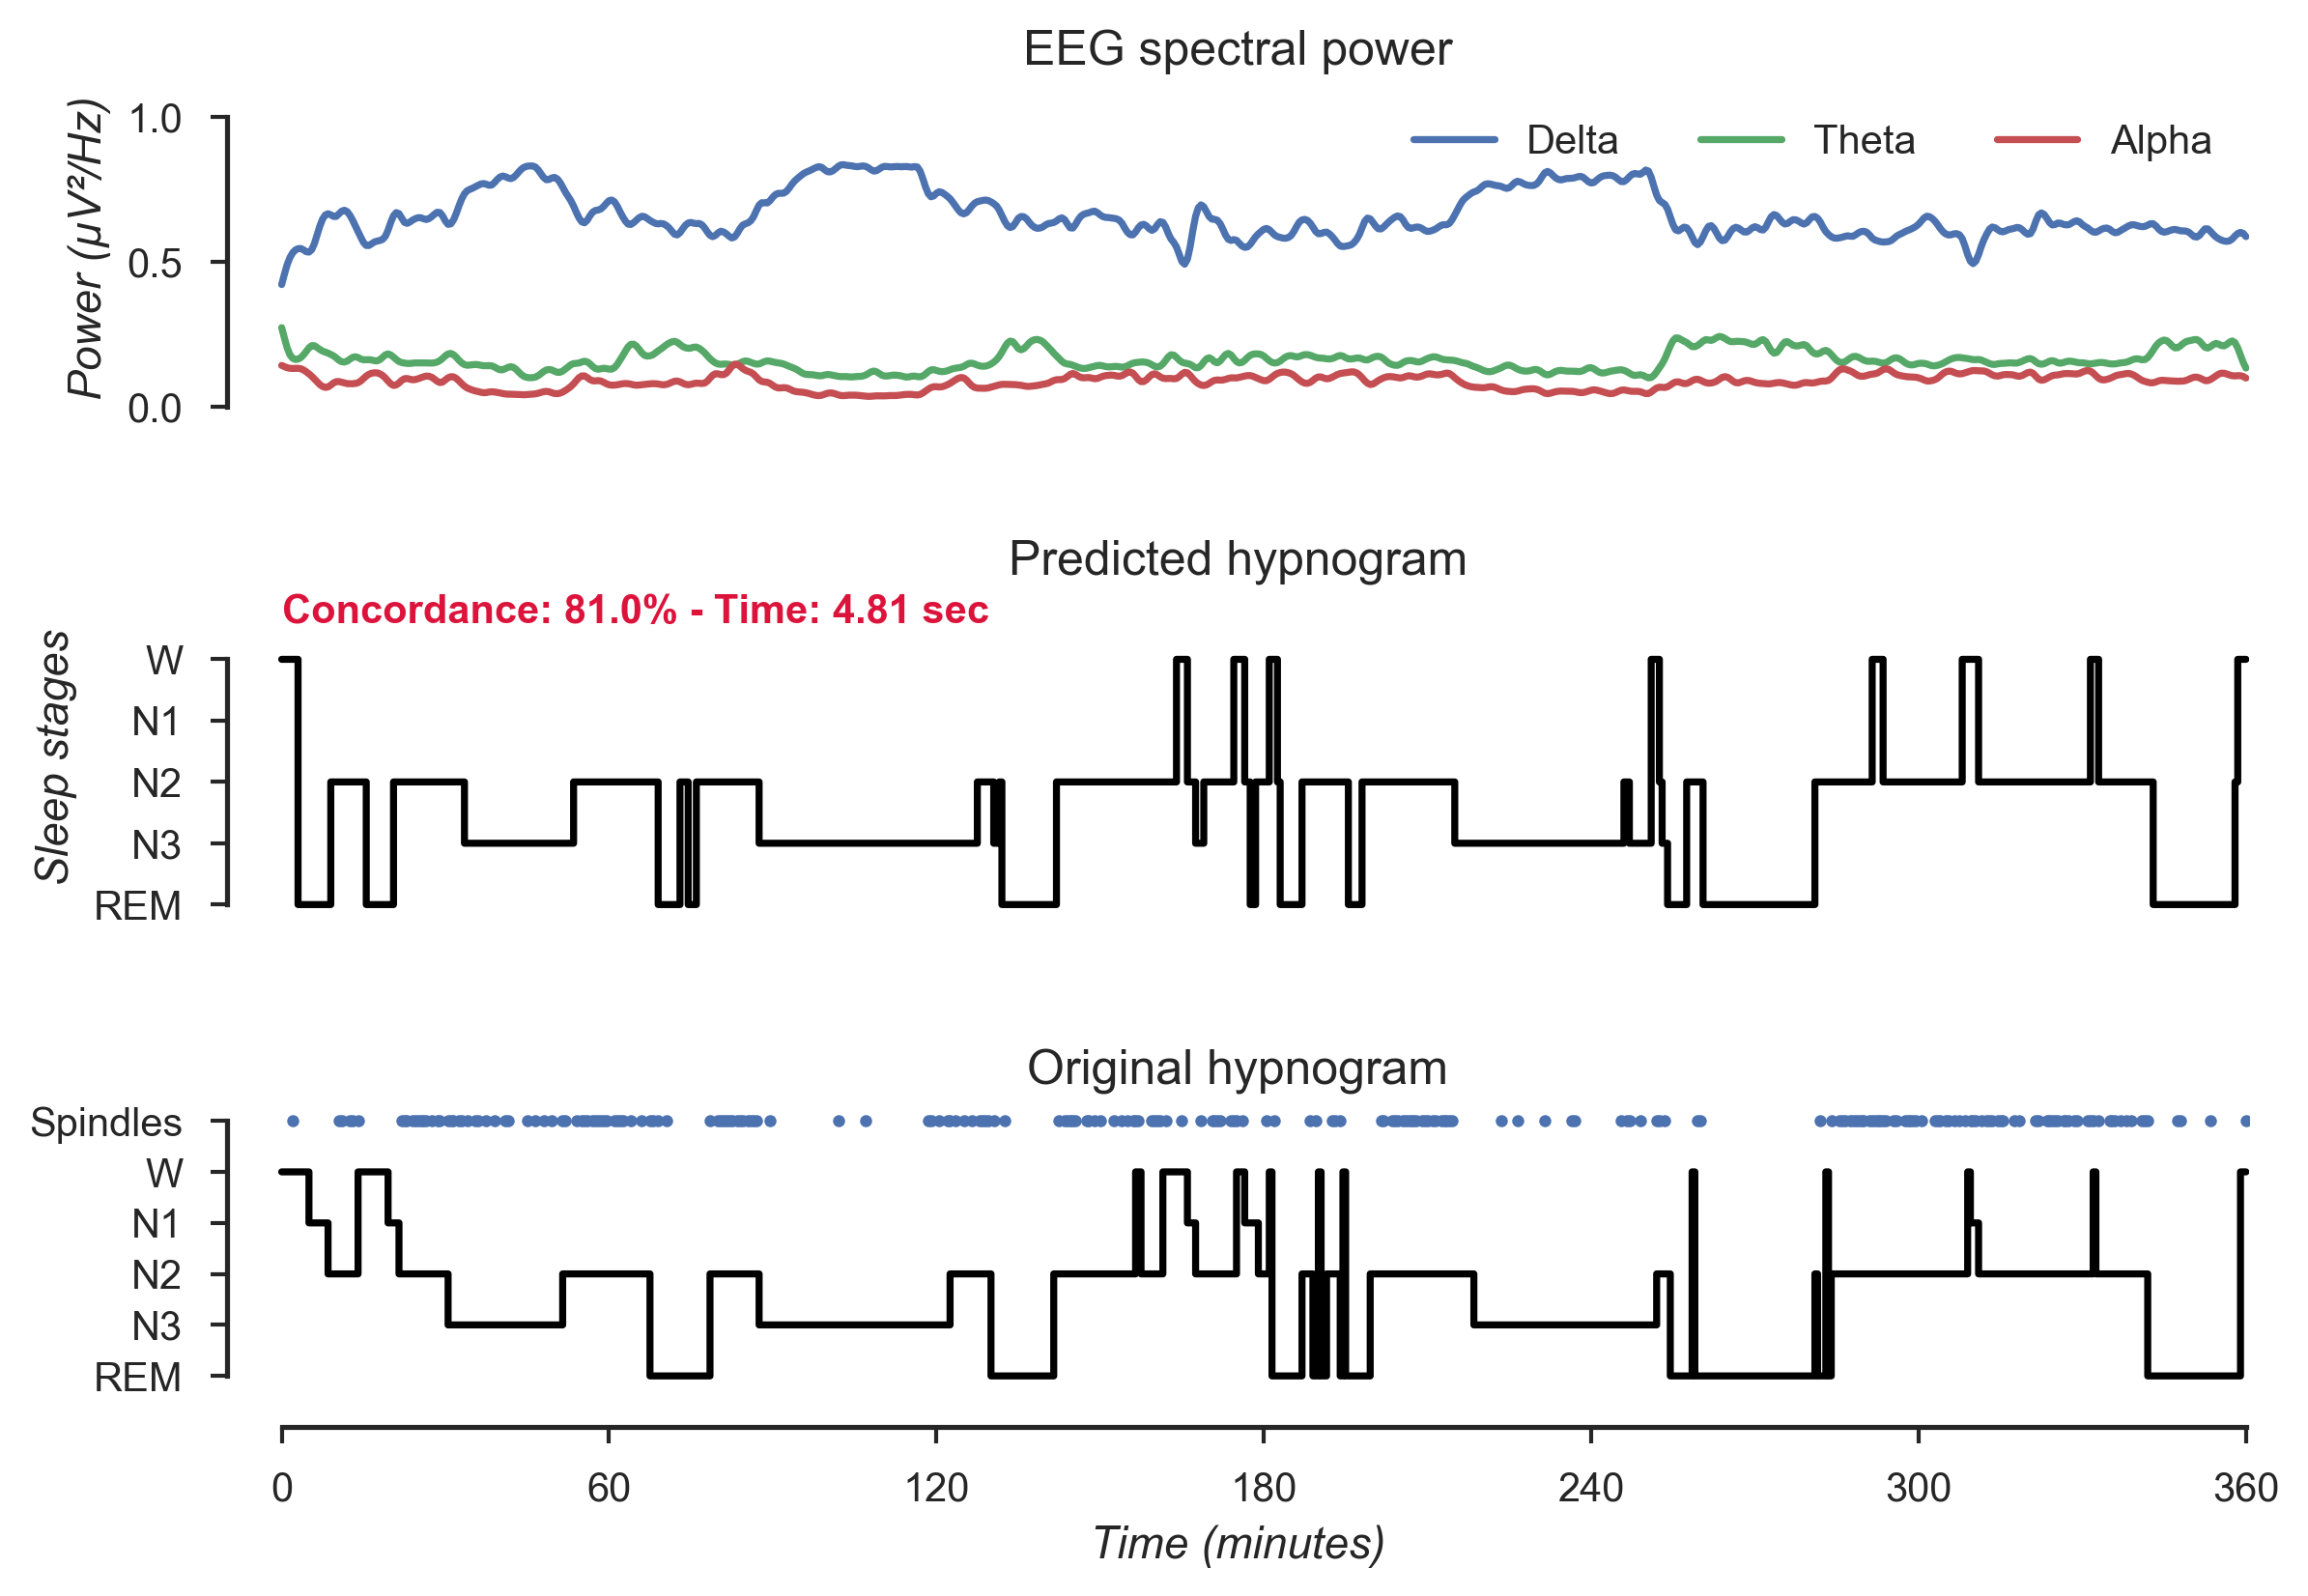
\includegraphics[width=\textwidth]{Fig/Discussion/autoscore.png}
	\caption[Preliminary results of the automatic sleep scoring algorithm]{Preliminary results of the automatic sleep scoring algorithm. The algorithm is based on a combination of spectral features extraction (Top) and automatic detection of microstructural features (e.g. spindles, blue dots).Preliminary tests on a full night PSG recording obtained on a healthy individual, using a single central derivation (C3), showed a percentage of concordance between the predicted and the manually scored hypnogram superior to 80\% (with a running time inferior to 5 seconds).}
	\label{fig:disc:methods:future:autoscore}
\end{figure}

Because this software represents one of the very few open-source, free and exhaustive solution for sleep reading, scoring and analysis, it should reach the broadest public (including sleep researchers, students, engineers) and lead to many great collaborations. In addition, the wide range of natively supported file formats makes it possible for numerous sleep laboratories across the world to visualize and analyze their sleep data using a single, common software. For all these reasons, the development of SLEEP represents a major step forward in sleep research, and more broadly, in open science.


%%%%%%%%%%%%%%%%%%%%%%%%%%%%%%%%%%%%%%%%%%%%%%%%%%%%%%%%%%%%%%%%%%%%%%%%%%%%%%%
\cleardoublepage
\chapter{General conclusion}
\label{disc:conclusion}
